\documentclass{ecai2014}
\usepackage{graphicx, latexsym, epstopdf, setspace, units, pgfplots, helvet, times, amsmath, mathtools, tabularx, booktabs}
\usepackage[algo2e, noend, noline, linesnumbered]{algorithm2e}
\DontPrintSemicolon
\newcommand\todo[1]{\textcolor{red}{#1}}
\newcommand{\pushline}{\Indp}% Indent
\newcommand{\popline}{\Indm}
\newcommand{\sgn}{\mathop{\mathrm{sgn}}}
\newcommand{\tuple}[1]{\ensuremath{\left \langle #1 \right \rangle }}
\newcommand{\node}[1]{{\fontfamily{phv}\selectfont#1}}
\newcommand{\E}[1]{\mathrm{E}\left( #1 \right)}
\newcommand{\Var}[1]{\mathrm{Var}\left( #1 \right)}
\newcommand{\Cov}[1]{\mathrm{Cov}\left( #1 \right)}
\newcommand{\Corr}[1]{\mathrm{Corr}\left( #1 \right)}
\newcommand{\defeq}{\vcentcolon=}
\pgfplotsset{compat=1.9}
\setlength{\belowcaptionskip}{-15pt}
\ecaisubmission   % inserts page numbers. Use only for submission of paper.
                  % Do NOT use for camera-ready version of paper.

\begin{document}

\title{Quality-based Rewards for \\ Monte-Carlo Tree Search Simulations}

%\author{Tom Pepels \and Mandy~J~.W. Tak \and Marc Lanctot \and Mark~H.~M. Winands \institute{Maastricht University, Department of Knowledge Engineering, Maastricht, The Netherlands, email: \{tom.pepels,mandy.tak,marc.lanctot,m.winands\}@maastrichtuniversity.nl} }

\maketitle
\bibliographystyle{ecai2014}

\begin{abstract}
Monte-Carlo Tree Search is a best-first search technique based on sampling the state space of a domain. In gameplay, positions are scored based on the rewards of numerous randomized play-outs. Generally, play-out rewards are defined discretely, e.g. $r \in \{-1, 0, 1\}$ and backpropagated from the expanded leaf to the root node. However, a play-out may provide additional information beside the loss/draw/win state of the terminal position. Therefore, we introduce measures for assessing the a posteriori quality of Monte-Carlo simulations. We show that altering the rewards of simulated play-outs based on their assessed quality improves results in five distinct two-player games. To achieve these results we propose two enhancements, the \emph{Relative Bonus} and \emph{Qualitative Bonus}. Both are used as control variates, a variance reduction method for statistical simulation. The former is based on the number of moves made during a simulation, whereas the latter relies on a domain-dependent assessment of the game's terminal state. The proposed enhancements lead to a performance increase in all five domains discussed.
\end{abstract}

%-------------------------------------------------------------------
\section{INTRODUCTION}
\label{sec:intro}
Monte-Carlo Tree Search (MCTS) is a search method based on random sampling of a domain \cite{coulom2007efficient,kocsis2006bandit}. MCTS grows a search tree online by selecting nodes to expand based on a selection policy. Rewards stored at nodes are averaged over the results of numerous simulations. Each simulation consist of two parts, 1) the selection step, where moves are selected and played according to the a selection policy, and 2) the play-out step, where moves are played according to a simulation policy. At the end of each play-out a terminal state is reached and the result $r$, usually expressed numerically in some discrete range, e.g. $r \in \{-1, 0, 1\}$ representing a loss, draw or win, respectively, is backpropagated along the tree from the expanded leaf to the root node. All rewards are colleced at the nodes on the first ply, on which the final move to play is based. The move is selected based on either the node with the highest number of visits, the highest average reward, or a combination \cite{chaslot2008progressive}. 

In this paper, two techniques are proposed for determining the quality of a simulation, based on properties of the play-out. The first, Relative Bonus, assesses the quality of a simulation based on its duration $d$. The second, Qualitative Bonus, considers a quality assessment of the terminal state $q$. Moreover, we show that adjusting $r$ in a specific way using $d$ or $q$ leads to increased performance in five distinct two-player games. Moreover, we determine the advantages of using the Relative Bonus in the General Gameplaying agent {\sc CadiaPlayer} \cite{bjornsson2009cadiaplayer}, which won the International GGP competition in 2007 and 2008.

Other techniques for rewarding simulations have been proposed \cite{Winands2011}, where play-outs are cut-off early and their state heuristically evaluated. Furthermore, evaluating the final \emph{score} of a game has shown to improve results in games that base the winning player on the one with the highest score \cite{shibahara2008combining}. However, for some domains a heuristic evaluation may not be available or too time-consuming, and certainly not all games determine the winning player on the highest scoring player. Nonetheless, by merely using the straightforward discrete reward $r$, any information other than the loss/draw/win state of the play-out's final position is disregarded. For these reasons, we propose assessing the rewards of play-outs based on any information available at a terminal state.

The paper is structured as follows. First, the general MCTS framework is discussed in Section \ref{sec:mcts}. Next, two different techniques for assessing the quality of play-outs are detailed. Section \ref{sec:qoreward} explains how rewards can be altered using the quality measures from Section \ref{sec:poqual}. Followed by pseudo-code outlining the proposed algorithm. Finally the performance of the proposed enhancements is determined in Section \ref{sec:experiments}, accompanied by a discussion and conclusion.

%-------------------------------------------------------------------
\section{MONTE-CARLO TREE SEARCH}
\label{sec:mcts}
\begin{figure}[ht]
	\centering
	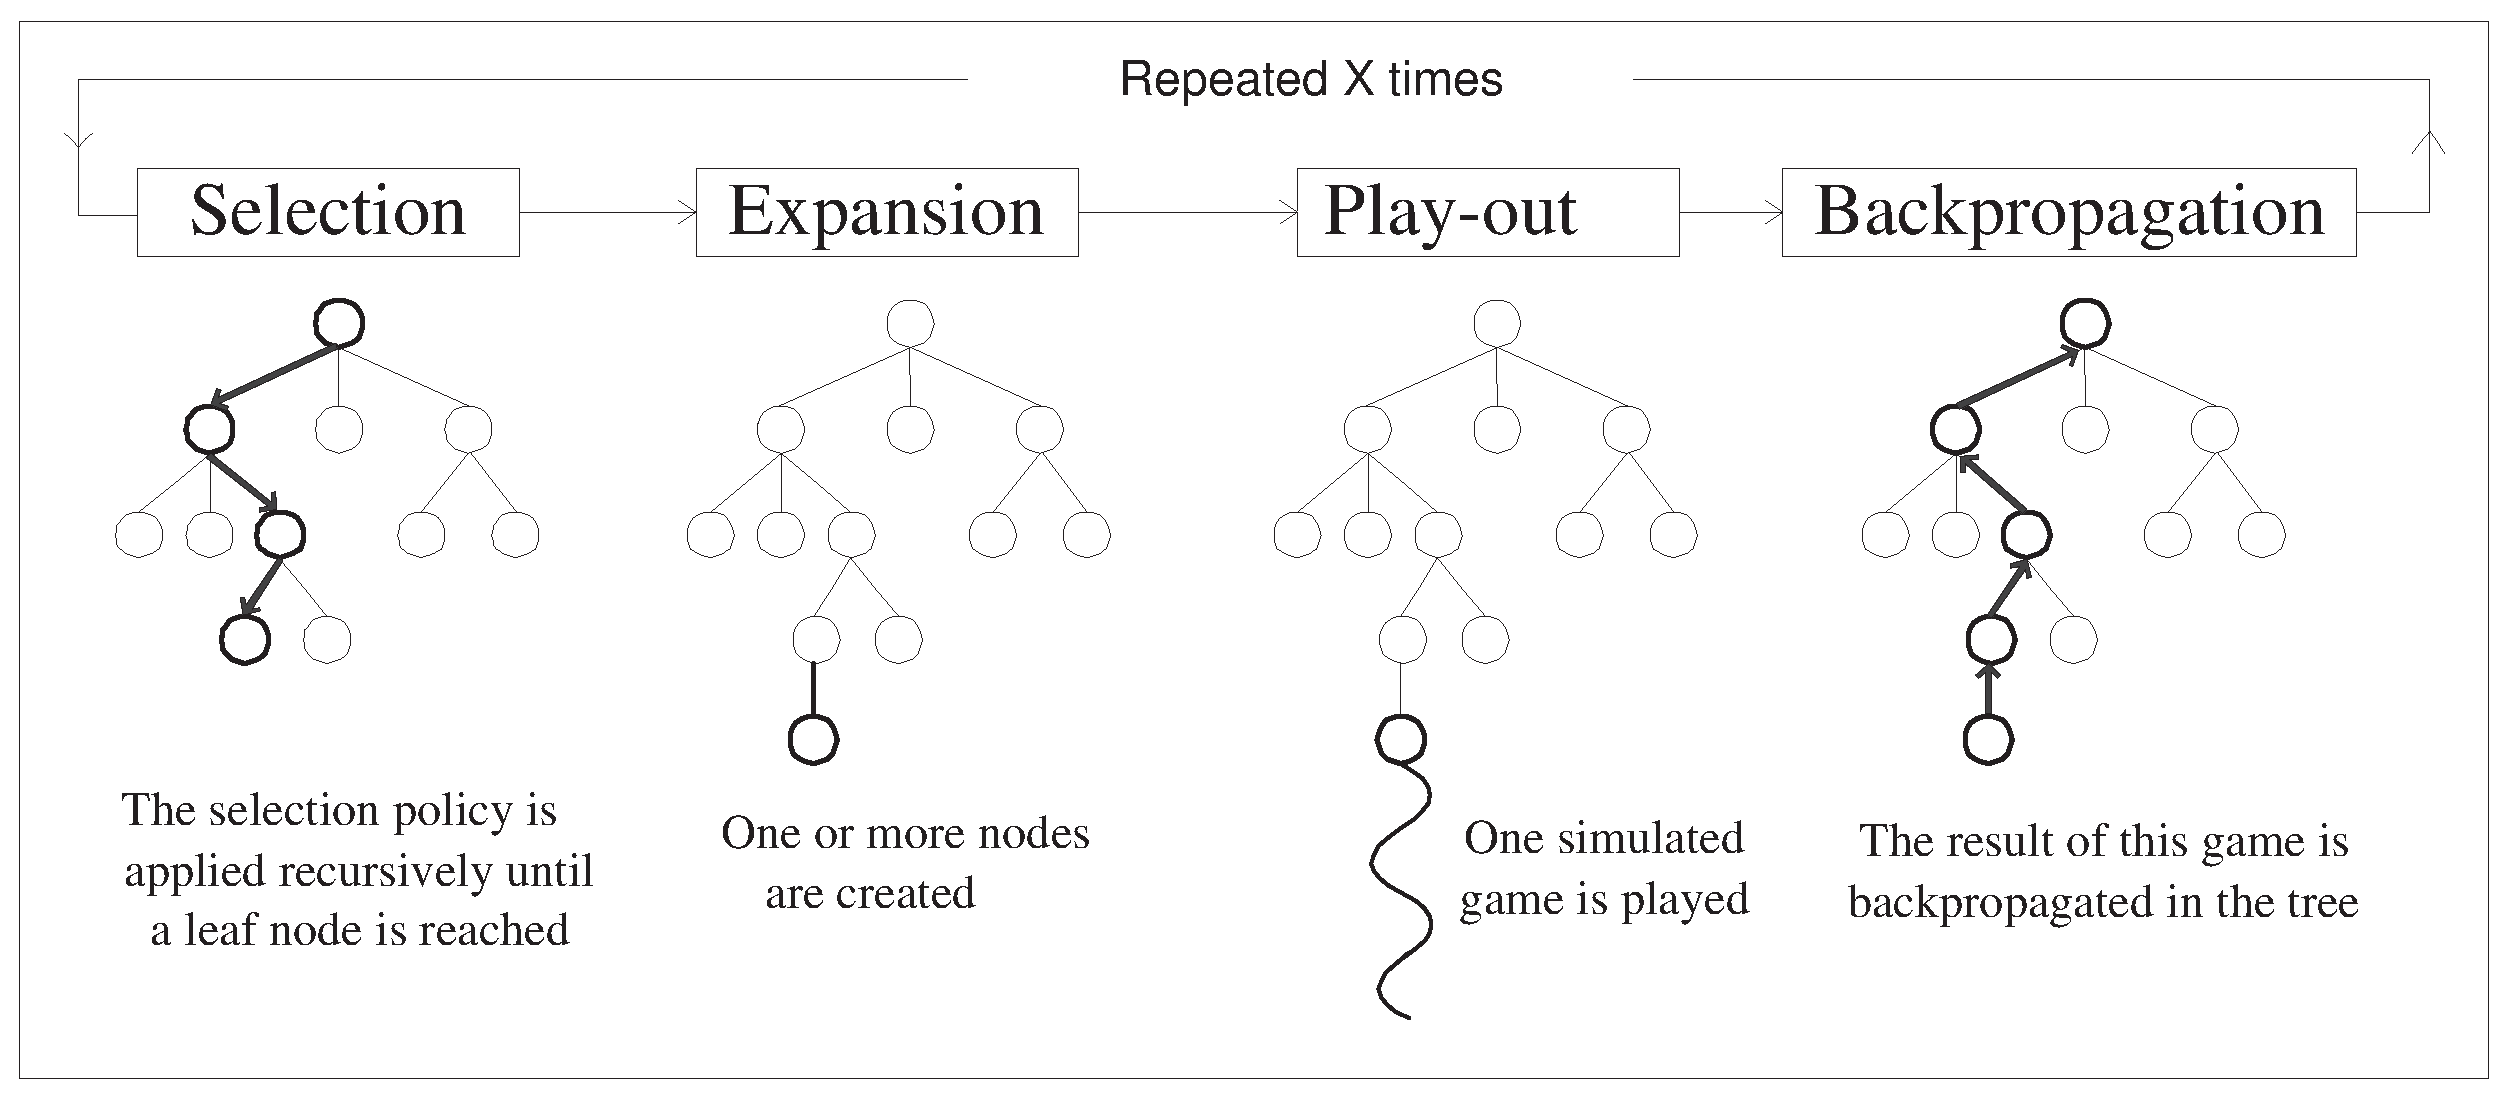
\includegraphics[width=.45\textwidth]{img/figure1.eps}
	\caption{Strategic steps of Monte-Carlo Tree Search \cite{chaslot2008progressive}.}
	\label{fig:mcts-algorithm}
\end{figure}

Monte-Carlo Tree Search (MCTS) is a best-first search technique based on random sampling of the state space for a specified domain \cite{coulom2007efficient,kocsis2006bandit}. In gameplay, this means that decisions are made based on the results of random play-outs. MCTS has been successfully applied to various two-player games games such as Go \cite{lee2010current}, Lines of Action \cite{Winands2010b}, and Hex \cite{arneson2010monte}. Moreover, MCTS has recently seen successes in other domains such as real-time strategy games \cite{browne2012survey}, arcade games such as Ms Pac-Man \cite{enhancementspacmancig12} and the Physical Travelling Salesman problem \cite{powleytsp}, but also in real-life domains such as optimization, scheduling and security \cite{browne2012survey}.

In MCTS, a tree is built incrementally over time. An average is maintained at each node corresponding to the rewards collected each time the node was visited. The root of the tree corresponds to the game's current position. The basic version of MCTS consists of four steps, which are performed iteratively until a computational threshold is reached, i.e. a set number of iterations, an upper limit on memory usage, or a time constraint. The four steps (depicted in Figure \ref{fig:mcts-algorithm}) at each iteration are \cite{chaslot2008progressive}:
\begin{itemize}
\item {\bf Selection.} Starting at the root node, children are chosen according to a selection policy described in Subsection \ref{subsec:uct}. When a leaf is reached that does not represent a terminal state it is selected for expansion.
\item {\bf Expansion.} All children are added to the selected leaf node given available moves.
\item {\bf Play-out.} A simulated play-out is run, starting from the state of the added node. Moves are performed randomly or according to a simulation policy until a terminal state is reached.
\item {\bf Backpropagation.} The result of the simulated play-out is propagated from the expanded node back up to the root. Statistics are updated along the tree for each node selected during the selection step and visit counts are increased accordingly.
\end{itemize}
The combination of moves selected during the selection and play-out steps form a single simulation. In its basic form, MCTS requires no evaluation function. Nonetheless, in most cases it is beneficial to add some domain knowledge for selecting moves to play during play-out. MCTS can be terminated anytime and select a move to play based on the number of visits or rewards  collected on the first ply.

%-------------------------------------------------------------------
\subsection{UCT}
\label{subsec:uct}
%from pac-man paper
During the selection step, a policy is required to explore the tree for rewarding decisions and finally converge to the most rewarding one. The Upper Confidence Bound applied to Trees (UCT) \cite{kocsis2006bandit} is derived from the UCB1 policy \cite{auer2002using} for maximizing the rewards of a multi-armed bandit. UCT balances the exploitation of rewarding nodes whilst allowing exploration of lesser visited nodes. Consider a node $p$ with children $I(p)$, then the policy determining which child $i$ to select:
\begin{equation}
\label{eq:uct}
i^* = argmax_{i \in I(p)}\left\{ v_i + C \sqrt{ \frac{\ln{n_p}}{n_i}}\right\}
\end{equation}
where $v_i$ is the score of the child $i$ based on the average result of simulations that visited it. $n_p$ is the visit count of the node and $n_i$ the visit count of the current child. $C$ is the exploration constant to be determined by experimentation.

\section{ASSESSING SIMULATION QUALITY}
\label{sec:poqual}
In this section two measures by which the quality of the terminal state of a simulation can be assessed are discussed. First, the duration of a simulation is discussed as a measure of its quality. Second, a quality assessment of the terminal state of a match is considered. In the next section we establish how these quantities can be used to enhance the rewards of MCTS simulations.

{\sc simulation duration} The first, straightforward assessment of a simulation's quality is the duration of the simulated game played. Consider a single MCTS simulation as depicted in Figure \ref{fig:mcts-simulation}, then we can define two seperate distances: 
\begin{enumerate}
\item The number of nodes between the root node \node{S} to the expanded leaf \node{N}, $d_{SN}$,
\item The number of moves required to reach \node{T}, the simulation's terminal state, from \node{N} during play-out $d_{NT}$.
\end{enumerate}
The length of the simulation is then defined as the sum of these distances:
\begin{equation}
d = d_{SN} + d_{NT}
\label{eq:m_ST}
\end{equation}
i.e. the total number of moves made by both players before reaching the terminal state of the game \node{T} from \node{S}, the root's game state.
\begin{figure}[t]
	\centering
	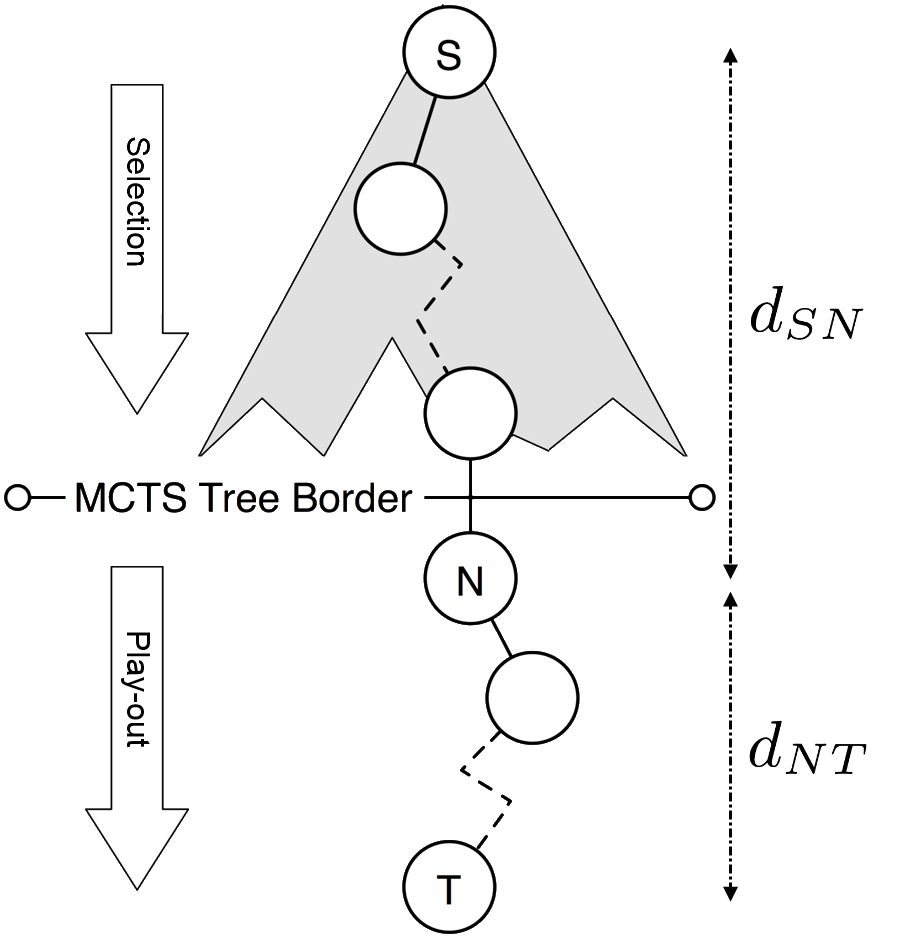
\includegraphics[width=.3\textwidth]{img/figure2_new.png}
	\caption{A single MCTS simulation \cite{finnsson2010learning}.}
	\label{fig:mcts-simulation}
\end{figure}
Moves played during play-out are selected by some simulation strategy. Generally this either a random strategy, or a rule-based, reactive strategy, combined with a source of randomness such as an $\epsilon$-greedy selection \cite{sturtevant2008analysis,sutton1998reinforcement}. Various alternative methods have been proposed, such as using low-level $\alpha\beta$ searches \cite{Winands2011}, and methods that learn a strategy online, such as N-Grams and the Last-Good-Reply policy \cite{Tak2012}, or the Move-average Sampling Technique (MAST) \cite{finnsson2008simulation}. However, each of these methods and strategies have some random element in common. Moreover, selected moves are far from optimal, because numerous simulations are to be made during the time allowed for search, any selection strategy cannot be made overly computationally intensive. As such, each move played ultimately increases uncertainty with respect to the accuracy of the final result by some degree. Hence, the duration of the simulation may be regarded as an indicator of the accuracy of its result.

The main benefit of using simulation duration as a quality measure is that it is domain independent. Unless the number of moves in the game is fixed, the duration of a play-out in particular can be informative in determining its quality. Moreover, in certain games such as Chinese Checkers, simulation length has already been considered part of the evaluation function \cite{roschke2013cc}. Thus it may be considered more than a mere property of the play-out.

{\sc terminal state quality} The second measure of a simulation's quality is based on a quality assessment of a match's terminal state. Although evaluation functions can be designed for most games, they're used to evaluate non-terminal states and assign them a specific value. However, this is contrary to MCTS, which generally performs a play-out until a terminal state is reached. Therefore, we are interested in evaluating the terminal state of a game rather than any intermediary states. Although this leaves potentially less informative features to be evaluated, it provides a direct application to MCTS.

As before, consider a single MCTS simulation as depicted in Figure \ref{fig:mcts-simulation}. When a terminal state is reached, a quality assessment function is called to evaluate the position with respect to the winning player. This measure $q$ should reflect the quality of a terminal state. For instance, in a game with material such as Breakthrough, Chess or Checkers, an evaluation can be based on scoring the remaining material of the winning player. For a racing game such as Chinese Checkers, the inverse of the number of pieces the opponent has in his target base can be considered. As such, the quality is based on the a posteriori evaluation of the terminal state. Having witnessed the states and actions performed from \node{S} to \node{T}, the score is based on an assessment of \node{T} given the progression \node{S} \ldots \node{N} \ldots \node{T} (see Figure \ref{fig:mcts-simulation}).

%-------------------------------------------------------------------
\section{QUALITY-BASED SIMULATION REWARDS}
\label{sec:qoreward}
Based on the classification of quality measures in the previous section, we propose two reward alterations for MCTS: \emph{Relative Bonus (RB)} and the \emph{Qualitative Bonus (QB)}, relating to the length of simulations and the quality assessment of terminal states, respectively. 

In the proposed framework, MCTS simulations return a tuple of four reward values, $\tuple{r,\tau,q,d_{NT}}$ representing the outcome $r\in\{-1, 0, 1\}$, the winning player $\tau$, the quality assessment of the terminal state $q\in(0, 1)$, and the distance from the expanded node \node{N} to the terminal state \node{T}, $d_{NT}$, respectively. $d\in(0, m)$ is then computed as shown in Equation \ref{eq:m_ST}, which is upper-bounded by the theoretical maximum duration of the game $m$. Apart from $q$, these values are available without requiring extra computational effort.

This section discusses the mathematical basis for altering MCTS rewards. Control variates as a means of variance reduction are discussed and how they can be used to improve MCTS' performance in games. In the second subsection the Relative Bonus is defined, based on the value of $d$. And the following subsection details the Qualitative Bonus, which is similar to RB aside from being based on the quality measure $q$. To conclude, we introduce a method for determining $a$, a constant used in the propsed methods.

\subsection{Control Variates}
Variance reduction methods in mathematical simulation are used to improve estimates by reducing the variance in a simulation's output \cite{kelton2000simulation}. Recently, using variance reduction techniques for MCTS has been proposed by Veness et. al. \cite{Veness11variance}. They applied, among others, control variates to UCT in different stochastic games to improve results by the reduction of variance in the reward signal. \todo{Say how our approach differs from theirs.}

Control variates take advantage of a possible correlation between two random variables $X$ and $Y$, to improve the estimate $\E{X}$ given that the mean $v=\E{Y}$ is known. This is achieved by adding the deviation of $Y$ from its mean, scaled by a constant $a$, to $X$. Which results in a new, controlled estimator $Z\defeq X+a\left(Y-v\right)$. For $a$, one can derive an optimal constant $a^*=-\Cov{X,Y}\mathbin{/}\Var{Y}$ such that the reduction in variance is optimal.

If we define $X$ as the simulation output, i.e. $X_n=r$, and define $Y$ as as one of the quality measures discussed in Section \ref{sec:poqual}, $Y_n=d$ or $Y_n=q$. Then assuming that $X$ and $Y$ are correlated, i.e. $\Corr{X,Y}\neq0$, we can find an optimal $a^*$ such that variance in the reward will be reduced. In common practical domains, no fixed values for $v$, $\Cov{X,Y}$, or $\Var{Y}$ are known and appropriate estimators for these quantities are required

Although using the quality measures as a control variates is appropriate for MCTS, it is not necessarily the case that optimal variance reduction results in optimal performance increase. In conclusion, although we expect that reducing the variance in the reward signal of MCTS benefits overall performance, it is not a guarantee. Moreover, it is possible that a larger performance increase is gained by using a non-optimal value for $a$, as our quality measures may provide more advantage than variance reduction alone. Therefore, althoug we propose to define quality-based rewards as control variates, we will not be concerned with the actual reduction in variance, but rather the improvement in performance.

\subsection{Relative Bonus}
\label{subsec:rb}
First, note that $d$ depends on both the domain and the progress of the game. By itself, the variable is neither normalized, nor relative to a central tendency over time. As such, using it as a control variate as is, leads to a biased distribution of the value over time, where, at the beginning of a game, $d$ takes on higher values than when the game nears its end. Moreover, considering that the length of a game cannot be determined beforehand, we have no accurate way of normalizing the observed values absolutely, based on the expected total length of the game. Therefore, $d$ is standardized as a \emph{t}-statistic. A sample mean can be approximated online, by maintaining an average $\bar{D}^\tau$ for each player (indexed by $\tau$), over the distribution of observed $d$ values $D^\tau$. After each simulation, $\bar{D}^\tau$ is updated with the observed $d$, then $\hat{\sigma}^\tau_D$ is the sample standard deviation of the distribution $D^\tau$. Using these statistics, we can define a standardized value $\lambda_r$ as follows:

\begin{equation}
\lambda_r = \frac{\bar{D}^\tau - d}{\hat{\sigma}^\tau_D}
\end{equation}

$\lambda_r$ is both normalized with the sample standard deviation, and is relative to $\bar{D}^\tau$. It is both independent of the progress of the game, and normalized with respect to the current variance in the length of simulations. The expectation of $\lambda_r$ values will be 0 due to standardization, hence $\lambda_r$ can be added to $r$ as a control variate with $v = 0$. Note that, values of $\lambda_r$ are higher for shorter simulations.

Using an estimated mean may cause the search to be biased, i.e. moving into the dierction of faster games. Although there is no immediate sollution to this problem, we propose to reset $\bar{D}^\tau$ and $\hat{\sigma}^\tau_D$ in between moves. Moreover, rewards of the first $5\%$ of the expected number of simulations are not altered during search, and $\bar{D}^\tau$ and $\hat{\sigma}^\tau_D$ are updated during this time without altered selection.

Since the distribution of $D^\tau$ is not known, $\lambda_r$ can still take on unrestricted values, particularly if the distribution of $D^\tau$ is skewed, or has long tails on either side. Moreover, the relation with the desired reward is not neccesarily linear. As such, in order to both bound, and shape the values of the bonus $b(\lambda_r)$ it is passed to a sigmoid function centered around $0$ on both axes. The range of the sigmoid is $[-a, a]$. Where $a$ can be an empirically optimized value, or computed off or on-line as described in the next subsection.

\begin{equation}
b(\lambda)=a\left(-1+\frac{2}{1+e^{-k\lambda}}\right)
\label{eq:sigmoid}
\end{equation}

$k$ is a constant to be determined by experimentation, it both slopes and bounds the bonus to be added to $r$. Higher values of $k$ determine both the steepness, and the start and end of the horizontal asymptotes of the sigmoid function. This type of function is commonly used to smooth reward values of evaluation functions. Moreover in \cite{shibahara2008combining} $r$ was replaced by a sigmoid representing the final score in Go.

Finally, the reward $r$ returned by the original simulation is yielded by $b(\lambda_r)$ as follows:
\begin{equation}
r_b=r+\sgn(r)\times b(\lambda_r)
\end{equation}

This value is backpropagated from the expanded leaf to the root node. The range of $r_b$ is now $[-1-a, 1+a]$, i.e. the bonus $b(\lambda)$ is centered around the possible values of $r$.

\subsection{Qualitative Bonus}
\label{subsec:qb}
Calculation of the Qualitative Bonus follows the same procedure as the Relative Bonus. Similar to RB, the average $\bar{Q}^\tau$ and standard deviation $\hat{\sigma}^\tau_Q$ of observed $q$ values is maintained for each player $\tau$. The value of $q$ is determined by an assessment of the quality of the match's terminal state. Assuming that higher values of $q$ represent a higher quality terminal state for the winning player $\tau$, $\lambda_q$ is defined as:
\begin{equation}
\lambda_q = \frac{q - \bar{Q}^\tau}{\hat{\sigma}^\tau_Q}
\end{equation}
Finally the bonus $b(\lambda_q)$ is computed using the sigmoid function in equation \ref{eq:sigmoid} with an optimized $k$ constant, and summed with the result of the simulation $r$.
\begin{equation}
r_q=r+\sgn(r)\times b(\lambda_q)
\end{equation}

\subsection{Estimating $a$}
\label{subsec:astar}

In gameplay, $X$ is a nominal variable, i.e. win, draw or loss, and $Y$ is a discrete scalar. Therefore the method of approximating $a^*$ by determining $-\Cov{X,Y}\mathbin{/}\Var{Y}$ is not straightforward, which may cause numerical issues. Also note that computing $a^*$ online based on the result of simulations depends heavily on the accuracy of the results of these simulations, and may cause the value of $a^*$ to be wrong or suboptimal. Furthermore, determining $a^*$ offline, fixes the value over the duration of the game, which is once again suboptimal because its value can be different over the course of the game, e.g. lower values at the start due to lower quality results.

The scaling constant for the defined control variates is dependent on the range of $r$, the simulation's result. Computing $a^*$, optimal for variance reduction, can thus be achieved by defining $X$ as $X_n=r$, if $r$ is in respect of one player, and $Y_n=d$ or $Y_n=q$. We can compute $a^*=-\widehat{\Cov{X,Y}}\mathbin{/}\widehat{\Var{Y}}$, i.e. using the sample covariance and variance, online during search, or offline. Regrettably, any effort to determine a value for $a$ based on the preceding method has been fruitless. Due to the small covariance measured the resuling range of $a$ is too small to make an impact on performance.

Nonetheless, a usable value for $a$, $a'$ can be computed and used online by altering the definition of $X$. First, let $Y$ be one of the proposed quality measured, i.e. $Y_n=r$ or $Y_n=q$. Let $\rho$ be the search player, i.e. the player running MCTS. Now, define $X'$ as:
\begin{equation}
X'_n =
\begin{cases}
   Y_n & \text{if $\rho$ wins the play-out,}, \\
   0   & \text{otherwise}
\end{cases}
\label{eq:xprime}
\end{equation}
$X'$ is then used to compute $\widehat{\Cov{X',Y}}$, and subsequently $a'$. \todo{Explain this}

%-------------------------------------------------------------------
\section{PSEUDO-CODE}

\begin{algorithm2e}[ht]
\setstretch{1.15}
  {\sc mcts}(node $p$, node depth $d_{Sp}$):												\;
  \pushline
    \If{isLeaf($p$)}{Expand($p$)}
    Select a child $i$ according to Eq.~\ref{eq:uct} 										\;
    $d_{Si} \gets d_{Sp} + 1$																\; \label{alg:depth}
    \eIf{$n_i = 0$}{
    	$\tuple{r, \tau, q, d_{iT}} \gets$ Playout$(i)$ 									\; \label{alg:results}
    	$d \gets d_{Si} + d_{iT}$															\;			
    	\If{enabled$(b_r)$ and $\hat{\sigma}^\tau_D > 0$}{
    		$r \gets r + \sgn(r) \times$ BONUS$(\bar{D}^\tau - d, \hat{\sigma}^\tau_D)$ 	\; \label{alg:rb}
    		update $\bar{D}^\tau$ and $\hat{\sigma}^\tau_D$ with $d$						\; \label{alg:meanstddev}
		}
		\ElseIf{enabled$(b_q)$ and $\hat{\sigma}^\tau_Q > 0$} {
    		$r \gets r + \sgn(r) \times$ BONUS$(q -\bar{Q}^\tau, \hat{\sigma}^\tau_Q)$ 		\; \label{alg:qb}
    		update $\bar{Q^\tau}$ and $\hat{\sigma}^\tau_Q$ with $q$ 						\;
    	}
    	update node $i$ with $r$															\;
    }{
    	$r \gets$ -{\sc mcts}($i$, $d_{Si})$)												\; 
    }
    update node $p$ with $r$																\;
   \popline
    {\bf return} $r$																		\;
  																							\;
    {\sc bonus}(offset from mean $\delta$, sample std. dev. $\hat{\sigma}$):				\;	\label{alg:bonus}
    \pushline
    	$\lambda \gets \nicefrac{\delta}{\hat{\sigma}}$										\;	\label{alg:lambda}
    	$b \gets a\left(-1+\nicefrac{2}{1+e^{-k\lambda}}\right)$							\;	\label{alg:b}
    \popline
    \bf{return} $b$																			\;
  \vspace{0.3cm}
  \caption{Pseudo-code of the MCTS and BONUS functions \label{alg}}
\end{algorithm2e}

Algorithm~\ref{alg} summarizes a single iteration of MCTS enhanced with RB and QB. Note that negamax backups are used in this setup, and therefore $r$ is relative to the player to move at the start of the play-out. Whenever and \emph{update} is used in the algoritm, it refers to updating the average reward for a node, or the sample mean and standard deviation for $\bar{D}^\tau$ and $\bar{Q}^\tau$. During selection, starting from the root, the depth of the current node is updated on line \ref{alg:depth}. Whenever an expandable node is reached, its children are added to the tree and a play-out is initiated from one of them. A play-out returns a tuple of results, on line \ref{alg:results} four different values are returned: 1) the result of the play-out $r \in \{-1, 0, 1\}$, 2) the winning player $\tau$, 3) the assessed quality of the play-out's terminal state $q\in(0,1)$, and 4) the number of moves made during play-out $d_{iT}$ defined in Subsection~\ref{sec:qoreward}. Using these values $r$ is altered. On line \ref{alg:rb} the relative bonus is applied to $r$, using the difference with the winning player's current mean $\bar{D}^\tau - d$, i.e. lower values of $d$ give a higher reward. After which the current mean and standard deviation are updated on line \ref{alg:meanstddev}. QB is applied on line \ref{alg:qb} using the assessed quality of the play-out $q$. Note that the offset from the mean is defined as $q - \bar{Q}^\tau$, because in contrast to RB, positive deviation of $q$ from its mean imply better results. The {\sc bonus} function on line \ref{alg:bonus}, computes the normalized $\lambda$ (line \ref{alg:lambda}) and, successively the bonus $b$ (line \ref{alg:b}) using the sigmoid function, as defined in Subsections \ref{subsec:rb} and \ref{subsec:qb}. The constant $a$ can be either fixed, or computed online.

%-------------------------------------------------------------------
\section{EXPERIMENTS}
\label{sec:experiments}
To determine the impact on performance of RB and QB, experiments were run on five different two player games. Moreover, the performance of RB is evaluated in the General Gameplaying agent {\sc CadiaPlayer} \cite{bjornsson2009cadiaplayer}, which won the International GGP competition in 2007 and 2008. 

\subsection{Experimental setup}
\label{subsec:expsetup}
The proposed enhancements were tested in five distinct two player games.
\begin{itemize}
\item \emph{Amazons} is played on a 10 x 10 chessboard. Each player has four amazons that move (and shoot) as queens in chess. However, each move consist of two parts, first the amazon moves, after which she must fire an arrow on an empty position in range, and this square on the board is blocked. The last player to move wins the game.
\item \emph{Breakthrough} is played on an 8 x 8 board. Each player starts with 16 pawns on one side of the board and the aim is to move one of them to the opposite side.
\item \emph{Cannon} is a chess-like game where the goal is to checkmate your opponents immobile town. Each player has one town he must place at the start of the game, and 15 soldiers. Soldiers can move or capture forward or may retreat if next to an opponent's soldier. Moreover, three soldiers in a row form a cannon that can move and shoot across the board.
\item \emph{Checkers} is played on an 8 x 8 board, and the goal is to capture all opponent's pieces.
\item \emph{Chinese Checkers} is played on a star shaped board. Each player starts with six pieces placed in one of the star's points, and the aim is to move all six pieces to the opposite side of the board. This is a variation of the original Chinese Checkers which is played on a larger board with 10 pieces per player.
\item \emph{Pentalath} is a connection game played on a hexagonical board. The goal is to place 5 pieces in a row. Pieces can be captured by fully surrounding an opponents set of pieces.
\end{itemize}
For the value of $q$ the following quality measures are used: \emph{Amazons}: the combined number of moves available for the winning player. \emph{Breakthrough} and \emph{Cannon}: the total piece difference between the winning and losing player. \emph{Checkers}: the total number of pieces in play for the winning player. \emph{Chinese Checkers}: the inverse number of the losing player's pieces that reached the home-base. \emph{Pentalath}: the inverse of the longest row of the losing player, given that this row can be extended to a length of 5.
For each quality measure an appropriate fixed, normalizer was used to bring the measure within the $(0,1)$ range.

All experiments were run on 2.2Ghz AMD Opteron CPU, on a Linux operating system. For each game, the constant $k$ used by the sigmoid function was empirically determined by experimenting with values between 0 and 10, with varying increments.
\subsection{Results}
\label{subsec:results}

\begin{table}
{\caption{Relative Bonus, 5000 games, 1 sec. per move.} \label{tab:rb}}
\begin{center}
\begin{tabular}{rlrrrr}
\hline
\rule{0pt}{12pt}
&&\multicolumn{2}{c}{\textbf{Online $a'$}}&\multicolumn{2}{c}{\textbf{$a$ = 0.25}} \\
\cline{3-6}
\rule{0pt}{12pt}
\textbf{Game} & \multicolumn{1}{c|}{\textbf{k}} & \textbf{Win \%} & \textbf{95\% c.i.} &\textbf{Win \%} & \textbf{95\% c.i.}\\
\hline
\rule{0pt}{10pt}
Amazons &\multicolumn{1}{l|}{2.2}			& 54.74\% & 1.38\% & \% & \% \\
Breakthrough &\multicolumn{1}{l|}{8.0} 		& 50.04\% & 1.39\% & \% & \% \\
Cannon &\multicolumn{1}{l|}{3.0} 			& 62.83\% & 1.34\% & \% & \% \\
Checkers &\multicolumn{1}{l|}{2.8}			& 52.11\% & 0.79\% & \% & \% \\
Chinese Checkers &\multicolumn{1}{l|}{1.2} 	& 56.76\% & 1.37\% & \% & \% \\
Pentalath &\multicolumn{1}{l|}{1.0} 		& 51.44\% & 1.39\% & \% & \% \\
\hline
\end{tabular}
\end{center}
\end{table}

\begin{table}
{\caption{Qualitative Bonus, 5000 games, 1 sec. per move.} \label{tab:qb}}
\begin{center}
\begin{tabular}{rlrrrr}
\hline
\rule{0pt}{12pt}
&&\multicolumn{2}{c}{\textbf{Online $a'$}}&\multicolumn{2}{c}{\textbf{$a$ = 0.25}} \\
\cline{3-6}
\rule{0pt}{12pt}
\textbf{Game} & \multicolumn{1}{c|}{\textbf{k}} & \textbf{Win \%} & \textbf{95\% c.i.} &\textbf{Win \%} & \textbf{95\% c.i.}\\
\hline
\rule{0pt}{10pt}
Amazons &\multicolumn{1}{l|}{1.6}			& 64.52\% & 1.33\% & \% & \% \\
Breakthrough &\multicolumn{1}{l|}{2.0} 		& 74.84\% & 1.20\% & \% & \% \\
Cannon &\multicolumn{1}{l|}{4.0} 			& 65.93\% & 1.31\% & \% & \% \\
Checkers &\multicolumn{1}{l|}{2.0}			& 53.82\% & 0.76\% & \% & \% \\
Chinese Checkers &\multicolumn{1}{l|}{2.8} 	& 65.70\% & 1.32\% & \% & \% \\
Pentalath &\multicolumn{1}{l|}{1.6} 		& 46.64\% & 1.38\% & \% & \% \\
\hline
\end{tabular}
\end{center}
\end{table}

%-------------------------------------------------------------------
\section{CONCLUSION}
Monte-Carlo Tree Search (MCTS) bases decisions on sampling a domain and collecting rewards. So far, not much work has been done to improve the values of the reward signal. In this paper, we show that the performance of MCTS is improved by treating the rewards of simulations as a combination of the reward and a quality measure. The combination is performed by treating the quality measure as a control variate, a variance reduction technique. We show that, given that there is a non-zero correlation between the reward-signal and the quality measure, results can be improved in two player games.
First, the Relative Bonus (RB) treats the length of a simulation as a measure of its quality. A benefit of this method is that it requires no domain knowledge. Although it works best in games with long play-outs, favoring the shorter ones. When the length of simulations is close to the lenght of the match played, RB provides less extra information, and therefore lesser performance enhancements. RB is especially interesting for General Game Playing (GGP), where knowledge of games is sparse, though in its current state is dependent on the $k$ parameter, which differs between games.
The Quality Bonus (QB) improved results in all domains, but requires a some extra domain knowledge. Nonetheless, even using simple quality assessment of the terminal state, such as the piece difference between players, improves results considerably.

%-------------------------------------------------------------------
\ack This work is partially funded by Scientific Research (NWO) in the framework of the project Go4Nature, grant number 612.000.938.

\bibliography{references}

\end{document}